\documentclass[]{article}
\usepackage[a4paper, margin=0.5in]{geometry}
\usepackage{graphicx}
\usepackage{amsmath}
\usepackage{amssymb}

%opening
\title{Solution for Problem Set F}
\author{
	Beshoy Saad, 2572741\\
	Rutuja Saptarshi, 2572864\\
	Vage Mkrtchyan, 2567128
}

\begin{document}
	
	\maketitle
	\section{Problem F1: B\"uchi Automata}
	\begin{itemize}
		\item [1] Briefly describe the difference between B\"uchi Automata and deterministic finite automata.
		
		For deterministic finite automates the word must end up in the final states of it (and naturally give no error while passing through the automate), then we determine that the word belongs to the automat. 
		\\
		\\
		\\
		In case of B\"uchi Automates, we are able to make claims about infinite words. We say that if the final state is met infinite times during the passing of the word through the automate, then the automate recognizes the word.
		
		\item [2] Find an LTL formula describing the words accepted by the following Büchi Automata with $\Sigma = \{a, b, c\}$ \\
		\begin{center}
			$G(((b \vee  c)Ua) \rightarrow ((bUc) \rightarrow G(b \vee  c))) \vee  G(b \vee c)$	
		\end{center}
		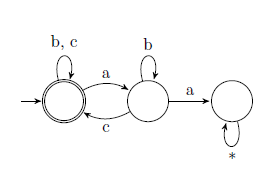
\includegraphics[scale=1]{A1.PNG}
		\begin{center}
			$(c \wedge  Xc) \vee (F(a \vee b)) \vee (F(a \vee b)U(c \wedge  Xc))$	
		\end{center}
		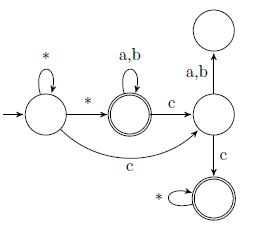
\includegraphics[scale=1]{A2.PNG}
		\begin{center}
			$(bUa)UF(bUc)$	
		\end{center}
		
		
		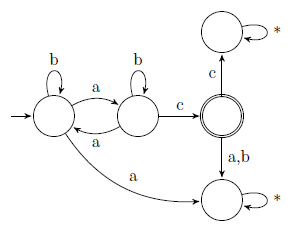
\includegraphics[scale=1]{A3.PNG}
	\end{itemize}
	
	\maketitle
	\section{Problem F2: Model Checking}
	\begin{itemize}
		\item [1] Region Graph\\
		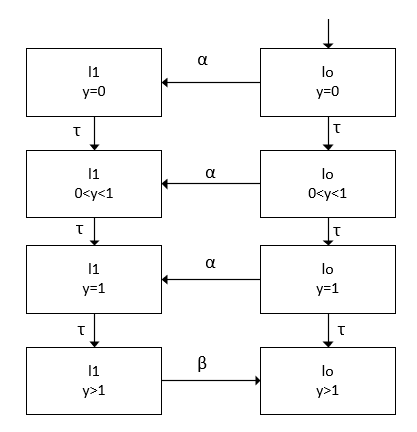
\includegraphics[scale=0.5]{RegionGraph.PNG}
		\item [2] Negating $\varphi$. \\
		$FG\neg{a}$ means that in the future the trace contains no as.
		$\neg{FG\neg{a}}$ - for every moment, there is an a in future.
		$$ \neg({FG\neg{a}}) = GFa$$
		\item [3] Construct a B\"uchi automaton $B_\varphi$.
		
		
		
		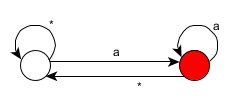
\includegraphics[scale=1]{p2.png}
		\item [4] 
	\end{itemize}
	
	\section{Problem F3: Reliability Analysis}
	\begin{itemize}
		\item [a] Overall reliability\\
		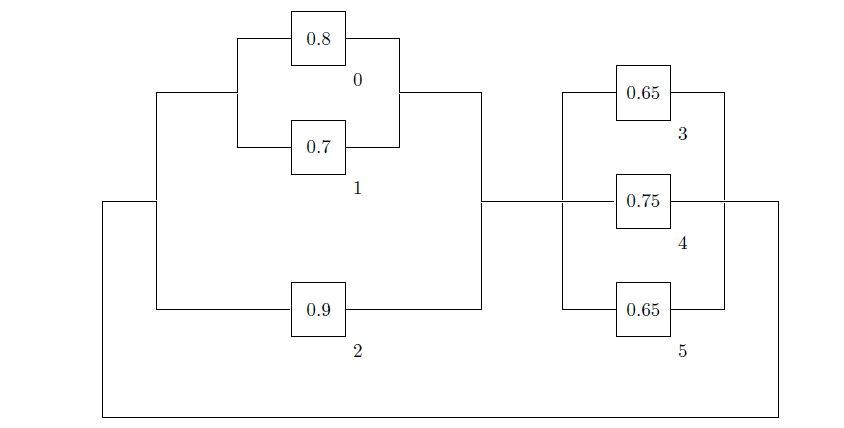
\includegraphics[scale=0.5]{F3}\\
		Simplifying the above system:\\
		\begin{align*}
			R_{A}(t)&=1-[(-R_0(t))(1-R_1(t))]\\
			&=1-[(1-0.8)(1-0.7)]\\
			&=1-[(0.2)(0.3)]\\
			&=1-0.06\\
			&=0.94
		\end{align*}
		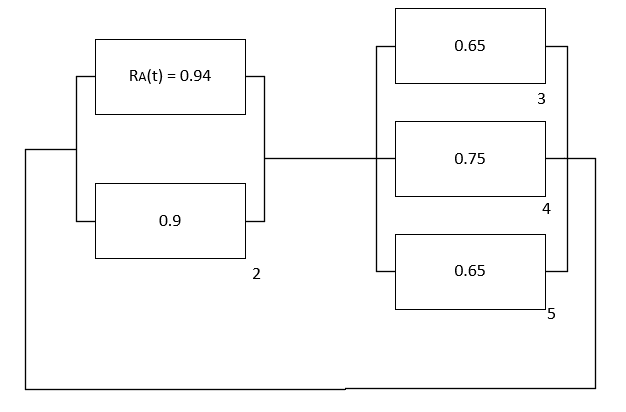
\includegraphics[scale=0.5]{Ra}\centering
		\begin{align*}
			R_{B}(t)&=1-[(1-R_{A}(t))(1-R_{2}(t)]\\
			&=1-[(1-0.94)(1-0.9)]\\
			&=1-[(0.06)(0.1)]\\
			&=0.994
		\end{align*}
		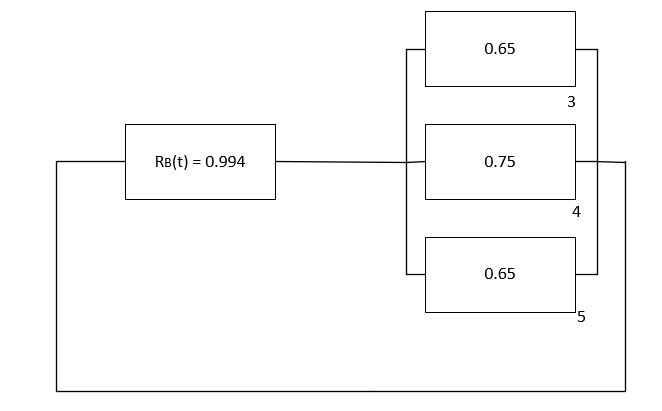
\includegraphics[scale=0.5]{Rb}
		\begin{align*}
			R_{C}(t)&=1-[(1-0.65)(1-0.75)(1-0.65)]\\
			&=1-[0.35*0.25*0.35]\\
			&=1-0.030625\\
			&=0.969375
		\end{align*}
		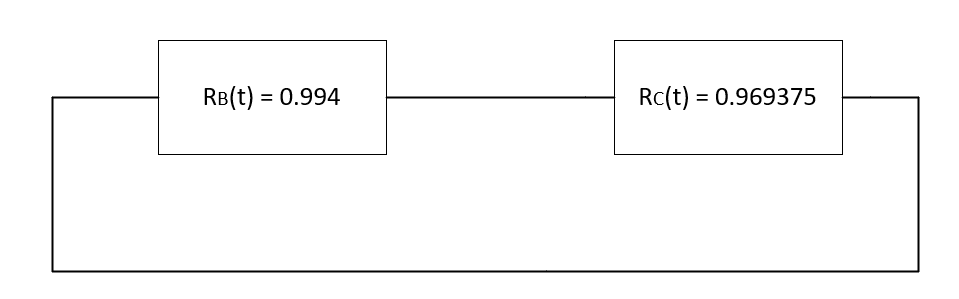
\includegraphics[scale=0.5]{Rc}
		
		\begin{align*}
			R(t)&=R_B(t) + R_C(t)\\
			&=0.994+0.969375\\
			&=0.96355875\\
			&=96.355\%
		\end{align*}
		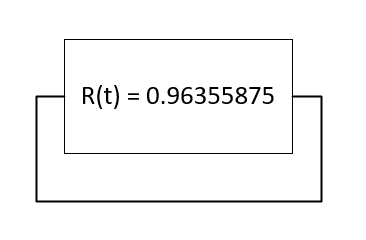
\includegraphics[scale=0.5]{Rt}\\
		
		\begin{flushleft}
			\item [b] The set S of all minimal cut sets of the given system is\\
			$S=[(block(0) and block(1) and block(2)] or [block(3) and block(4) and block(5)]$
			
			\item [c] Lower bound is given by\\
			\begin{align*}
				R(t)&\geqslant1 - \sum\pi(1-R_i(t))\\
				&\geqslant1-\Big\{\big[(1-0.8)(1-0.7)(1+0.9)+(1-0.65)(1-0.75)(1+0.65)\big]\Big\}\\
				&\geqslant1-\Big\{(0.2*0.3*0.1)+(0.35*0.25*0.35)\Big\}\\
				&\geqslant1-\Big\{0.006+0.030625\Big\}\\
				&\geqslant	1-0.036625\\
				&\geqslant 0.963375\\
				&\geqslant96.337%
			\end{align*}
			The exact bound computed before is more than the lower bound 
			
			\item [d] One algorithm gives lower bound on the reliability of the system, while other one gives the exact value of reliability. We prefer the lower bound algorithm as it gives the lower cut off on the reliability for critical applications.
		\end{flushleft}
	\end{itemize}
	
	\section{F4: Deductive Verification}
	$@pre : \|s\|=len \wedge (\forall i:0  \textless len \Rightarrow s[i]\in[0,255]) $\\
	$@post : rv \Leftrightarrow (\sum_{i=0}^{len} s[i])len^{-1} \geqslant 200$\\
	Consider statement for the loop to be : $@L\quad0 \leqslant i \wedge [\forall j \quad0 \textless j \textless i \rightarrow acc\quad div\quad len \textless 200]$
	
	Step I:Basic paths
	\begin{itemize}
		\item [1] $@pre : \|s\|=len \wedge (\forall i:0  \textless len \Rightarrow s[i]\in[0,255]) $\\
		$S_1:i:=0$\\
		$S_2:accu:=0$\\
		$@L\quad0 \leqslant i \wedge [\forall j \quad0 \textless j \textless i \rightarrow acc\quad div\quad len \textless 200]$
		\item [2]  $@L\quad0 \leqslant i \wedge [\forall j \quad0 \textless j \textless i \rightarrow acc\quad div\quad len \textless 200]$\\
		$S_1:assume\quad i \textless len$\\
		$S_2:accu=accu+s[i]$\\
		$S_3:assume\quad accu \quad div \quad len \textless 200 $\\
		$S_4:i:=i+1$\\
		$@post : rv \Leftrightarrow (\sum_{i=0}^{len} s[i])len^{-1} \geqslant 200$\\
		\item [3] $@L\quad0 \leqslant i \wedge [\forall j \quad0 \textless j \textless i \rightarrow acc\quad div\quad len \textless 200]$\\
		$S_1:assume \quad i \textless len$\\
		$S_2:accu=accu+s[i]$\\
		$S_3:assume\quad accu \quad div \quad len \geqslant 200$\\
		$S_4:rv:=true$\\
		$@post : rv \Leftrightarrow (\sum_{i=0}^{len} s[i])len^{-1} \geqslant 200$\\
		\item[4] $@L\quad0 \leqslant i \wedge [\forall j \quad0 \textless j \textless i \rightarrow acc\quad div\quad len \textless 200]$\\
		$S_1:assume\quad i \geqslant 200$\\
		$S_2:avg:=accu \quad div \quad len$\\
		$S_3:res:avg \geqslant200$\\
		$S_4:rv:=res$\\
		$@post : rv \Leftrightarrow (\sum_{i=0}^{len} s[i])len^{-1} \geqslant 200$\\
	\end{itemize}
	Step II Compute VCs for each basic path
	calculate weakest precondition for 2:\\
	$wp(post,S_1;S_2;S_3;S_4)$\\
	$wp(wp(post,S_4),S_1;S_2;S_3)$\\
	$wp(wp(rv \Leftrightarrow (\sum_{i=0}^{len} s[i])len^{-1} \geqslant 200,i:=i+1),S_1;S_2;S_3)$\\
	$wp(wp((\sum_{i=0}^{len} s[i])len^{-1} \geqslant 200[i:=i+1],assume\quad accu \quad div \quad len \textless 200),S_1;S_2)$\\
	$wp(wp(\quad accu \quad div \quad len \textless 200 \rightarrow \sum_{i=0}^{len} s[i])len^{-1} \geqslant 200[i:=i+1],S_2);S_1)$\\
	$wp(wp(\quad accu \quad div \quad len \textless 200 \rightarrow \sum_{i=0}^{len} s[i])len^{-1} \geqslant 200[i:=i+1],accu=accu+s[i]);S_1)$\\
	$wp((\quad accu \quad div \quad len \textless 200 \rightarrow \sum_{i=0}^{len} s[i])len^{-1} \geqslant 200[i:=i+1][accu=accu+s[i]],assume\quad i \textless len)$\\
	$i \textless len \rightarrow \quad accu \quad div \quad len \textless 200 \rightarrow \sum_{i=0}^{len} s[i])len^{-1} \geqslant 200[i:=i+1][accu=accu+s[i]] $\\
	Hence, the VC is:\\
	$\quad0 \leqslant i \wedge [\forall j \quad0 \textless j \textless i \rightarrow acc\quad div\quad len \textless 200]$\\
	$\rightarrow$ $i \textless len \rightarrow \quad accu \quad div \quad len \textless 200 \rightarrow \sum_{i=0}^{len} s[i])len^{-1} \geqslant 200[i:=i+1][accu=accu+s[i]]$
	which is valid by inspection.
\end{document}
